\documentclass[12pt, twosides]{report}

\usepackage{graphicx}
\graphicspath{ {figures/} }
\usepackage[left=2.5cm,right=2cm,top=2.5cm]{geometry}


\usepackage[utf8]{inputenc}
\usepackage{t1enc}
\usepackage[magyar]{babel}
\linespread{1.5}

\usepackage{footnote}
\usepackage{subfigure}
\usepackage{float}
\usepackage[]{algorithm2e}
\usepackage{amsmath}
\usepackage{mathptmx}
\usepackage{pdfpages}

\usepackage{xcolor}
\usepackage{hyperref}
\hypersetup{
    colorlinks,
    linkcolor=black,
    citecolor=black,
	urlcolor={blue!80!black},
	unicode=true
}
% 
\urlstyle{same}

\usepackage{listings}
\definecolor{dkgreen}{rgb}{0,0.6,0}
\definecolor{gray}{rgb}{0.5,0.5,0.5}
\definecolor{mauve}{rgb}{0.58,0,0.82}
\definecolor{light-gray}{gray}{0.25}

\lstdefinestyle{yaml}{	
	backgroundcolor=\color{white}, % choose the background color;
	basicstyle=\fontsize{8}{8}\ttfamily,% the size of the fonts that are used for the code
	breakatwhitespace=false, % sets if automatic breaks should only happen at whitespace
	breaklines=true, % sets automatic line breaking
	commentstyle=\color{dkgreen},  % comment style
	deletekeywords={...},  % if you want to delete keywords from the given language
	escapeinside={\%}{)},  % if you want to add LaTeX within your code
	extendedchars=true,  % lets you use non-ASCII characters; for 8-bits encodings only, does not work with UTF-8
	frame=none,	 	 % adds a frame around the code
	keepspaces=true, % keeps spaces in text, useful for keeping indentation of code (possibly needs columns=flexible)
	keywordstyle=\color{blue}\bfseries, % keyword style
	otherkeywords={*,...}, % if you want to add more keywords to the set
	numbers=none,  % where to put the line-numbers; possible values are (none, left, right)
	numbersep=5pt, % how far the line-numbers are from the code
	numberstyle=\tiny\color{gray}, % the style that is used for the line-numbers
	rulecolor=\color{black}, % if not set, the frame-color may be changed on line-breaks within not-black text (e.g. comments (green here))
	showspaces=false,% show spaces everywhere adding particular underscores; it overrides 'showstringspaces'
	showstringspaces=false,  % underline spaces within strings only
	showtabs=false,  % show tabs within strings adding particular underscores
	%stepnumber=1,  % the step between two line-numbers. If it's 1, each line will be numbered
	stringstyle=\color{mauve}, % string literal style
	tabsize=2,
	columns=fullflexible  % Using fixed column width (for e.g. nice alignment)
	sensitive = true,
	morekeywords={name, runs-on, on, jobs, build, run, steps, uses}
}
\lstset{}

\title{
	{Sapi3D tour - UI}\\
	{\large Sapientia\\
	Erdélyi Magyar Tudományegyetem, Marosvásárhely}
}
\author{
	Nagy-Serbán, Tünde\\
	\texttt{nagy.serban.tunde@student.ms.sapientia.ro}
	\and
	Szántó, Zoltán\\
	\texttt{zoltan.szanto@ms.sapientia.ro}	
}
\date{2021}

%%%%%%%%%%%%%%%%%%%%%%%%%%%%%%%%%%%%%%%%%%%%%%%%%%%%%%%%%%%%%%%%%%%%%%%%%
\begin{document}


\includepdf[pages={1,2,3}]{pdfs/allamvizsgaBorito.pdf}

\section*{Extras}
Extract

\textbf{Cuvinte cheie}: 

\pagebreak


\includepdf[pages={6}]{pdfs/allamvizsgaBorito.pdf}

\section*{Kivonat}
A dolgozat egy webalkalmazást mutat be, amely a Sapientia Erdélyi Magyar Tudományegyetem Marosvásárhely-i karának a 3D virtuális túráját foglalja magába. 

A mai világban az emberek napjait nagyban befolyásolja a digitalizáció. A legtöbb embernél található legalább egy okostelefon, számítógép, laptop. Viszont nem elég, hogy a digitális eszközök nélkül az élet elképzelhetetlenné válik, mellette még ott van az Internet is. 

A digitalizáció az emberek számára nagyon sok jó dolgot vezet be. Rengeteg problémát tudunk megoldani az internet és a digitális eszközök segítségével, mint például: számlák fizetése, távoli rokonokkal könnyebb a kapcsolattartás és nem utolsó sorban a virtuális túrák segítségével eltudunk jutni olyan helyekre ahová nem biztos, hogy az életben lesz lehetőségünk.

A dolgozatban egy webes applikációról van szó amley felhasznál egy 3D modellt az egyetemről létrehozva az egyetem úgy nevezett virtuális túráját. A túrán bárki résztvehet ezáltal betekintést nyerhet az egyetem fala mögé. Ezen kívűl informatív jelleggel is rendelkezik, mivel az alkalmazás számos információt megjelenít az egyetemmel kapcsolatban, mint például: különböző események (Sapi-Line-Tracer), szakkoordinátorok nevei, elérhetőségei.

Az alkalmazás egyik legfontosabb funkciónalítása az úgy nevezett "Vigyél el!" funkciónalítás, amely magába foglalja azt, hogy a felhasználót virtuálisan körbe visszi az egyetemen. A felhasználó megmondja hová szeretne eljutni és az alkalmazás egy adott útvonalon bemutatja az oda vezető útat. Ezen kívül arra is van lehetőség, hogy a felhasználók saját maguk lépegessenek az egyetem modelljén így még jobban körbe tudják járni azt.

A rendszer webes felelületre készült és ennek köszönhetően majdnem minden eszközön meglehet tekinteni, úgy a számítógépen mint a laptopon és nem utolsó sorban a telefonon is. Az alkalmazás sok segítséget nyújthat az újjonnan érkező egyetemistáknak, vendég diákoknak és a vendég tanároknak is az egyetem fő épületében való eligazodásnál. 

\textbf{Kulcsszavak}: web, 3D modell, virtuális túra.
\pagebreak

\section*{Abstract}
Abstract

\textbf{Keywords}: 
\pagebreak

\pagenumbering{gobble}

\tableofcontents

\listoffigures

\chapter{Bevezető}
\pagenumbering{arabic}
\paragraph{}
A mai gyorsan fejlődő világunkban a digitális eszközök kezdik átvenni az uralmat. Nem sok olyan háztartás van ahol nincs egyáltalán legalább egy telefon, számítógép, laptop, okos tv stb. Az elmúlt években a digitális világ annyira fejlett lett, hogy lassan már ki sem kell mozdulnunk a házból és mindent eltudunk végezni. Például ki tudjuk fizetni a számláinkat, be tudunk vásárolni stb. Ezek mellett egyes múzeumokat, iskolákat, kastélyokat, látványosságokat is betudunk járni otthon a négy fal között a 3D virtuális túrák segítségével. De mit is jelent, mire is használják ezeket a 3D virtuális túra modelleket?
\paragraph{}
A 3D jelentése három dimenzió. Ez egy modell, amely tulajdonképpen matematikailag ábrázol egy háromdimenziós objektumot. Ez lehet épület, virág, ember stb. A 3D modelleket széles körben használják az orvostudományban, magasabb szintű gyakorlati és elméleti kompetenciák elérésében. A 3D modellekkel nem csak tárgyakat hanem emberi folyamatokat is le lehet szimulálni. Az orvos tudományban nagyon szépen letudják előre játszani az operációkat így biztosabban fognak neki az adott műtétnek mivel jobban tudják kezelni a kockázatokat. Ilyen modellek felhasználásával egy adott problémát is jobban betudnak mutatni az emberek számára. Ilyen példa lehet egy hajóforgalom szimulációs rendszer amely figyelembe veszi a hajókat, vízfelületet és az időjárási viszonyokat. Ezzel a rendszerrel próbálták megmutatni az olajszennyezést a tengerekben, óceánokban.\cite{dedov2017design} Ezen modellek segítségével a világ látványosságai elérhetővé válhatnak azon emberek számára is akik nem jutnak el az eredeti országba, városba, hogy megtudják tekinteni az adott látványosságot.
\paragraph{}
A tour (virtuális túra) szó jelentése utazás, kirándulás. A mai világban túrázni nem csak a való életben lehet hanem a virtuális világban is. Egy ilyen virtuális túra célja, hogy fejlettebb szimulációs technikák segítségével a nézők életképes 3D-s képet kapjanak a meglévő helyről. Egy híres és megemlítendő példa a Second-Life ahol a felhasználók közötti interakció avatárokon keresztül zajlik. Ez azért megemlítendő példa mivel ezen alkalmazáson belül interaktív 3D tour-ok vannak leképezve.\cite{moloo20163d}
\paragraph{}
A 3D és a tour(virtuális túra) szavak összetételéből jön ki a 3D tour(3D virtuális túra) amely azt tükrözi, hogy a virtuális világban tudunk megnézni adott épületeket, kilátásokat, látványosságokat. Világunk fejlődése próbálja biztosítani, hogy egyetlen ember se maradjon le azon helyekről ahová nem tud eljutni. Habár ezen virtuális 3D modelleken alapuló világ még nem tökéletes de folyamatosan fejlődik. A dolgozatomon belül egy ilyen modellről lesz szó amely a Sapientia Erdélyi Magyar Tudományegyetem Marosvásárhely-i karának egy részét tartalmazza. A projekt két részre van bontva. Egy személy készíti el maga a modellt míg egy másik társ a felhasználói felületet. Közös munka a modellel történő attrakciók megoldása. Ezen dolgozatban a felhasználói felületről lesz inkább szó. 
\paragraph{}
A projekt célja, hogy a felhasználók a saját házukból is betekintést tudjanak nyerni az egyetem falai mögé is. Ez elsősorban az új felvételizőknek és az első éves egyetemistáknak lenne hasznos, mivel ez által már otthon neki foghatnak áttekinteni az egyetem különböző részeit mint például, hogy hol található egy adott tanszék, vagy hol található a dékáni hivatal, vagy hogy hol található a pénztár. Úgy gondolom, hogy ez az alkalmazás hasznos tud lenni a diákok részére sőt a szakkoordinátorok dolgát is megtudja annyiban könnyíteni, hogy az újonnan érkező diákok nem kell mindig tőlük kérdezzék, hogy hol találnak meg egy adott részleget.
\paragraph{}
Több okot is fellehet sorolni annak érdekében, hogy miért is használatosak ezek a 3D modellekkel megalkotott virtuális túrák. Első sorban az új diákok már otthonról be tudnak nézni az egyetem falai mögé így amikor elérkeznek az új év kezdéséhez akkor otthonosabban érezhetik magukat. Ez azért történhet meg mert már fogják tudni, hogy mit hol találnak nem kell segítséget kérjenek. Egy másik ok, hogyha az adott egyetem rendelkezik egy ilyen típusú modellel akkor jobban felhívhatja a figyelmet a diákok számára. Ez által az egyetem népszerűsítése is megtörténik. Ismert, hogy egyes szülők nehezen engedik el gyermeküket egyetemre mert féltik. Viszont az, hogy látnak egy  képet az egyetemről megnyugtathatja őket így bátrabban biztathatják gyermeküket, hogy menjen el az adott egyetemre. 
\paragraph{}
Összefoglalva egy ilyen 3D modell amely az egyetemet ábrázolja és bemutatja hasznos lehet, az egyetem, a diákok és szüleik számára is. Egy ilyen alkalmazás esetében nem csak maga a modell jelenik meg hanem rajta kívül számos fontos információ, elérhetőség is. Dolgozatom célja bemutatni a Sapientia Erdélyi Magyar Tudományegyetem 3D Virtual Tour alkalmazás megalkotását, implementálását és nem utolsó sorban a felhasznált technológiákat



\chapter{Célkitűzések}
A projekt célja, hogy a felhasználók távolról is megtudják nézni az egyetemet. Ez elsősorban az új felvételizőknek és az első éves egyetemistáknak lenne hasznos, mivel ez által már otthon neki foghatnak áttekinteni az egyetem különböző részeit mint például, hogy hol található egy adott tanszék, vagy hol található a dékáni hivatal, vagy hogy hol található a könyvtár. Ilyen alkalmazás hasznos lehet úgy a diákok mint a tanárok, szakkoordinátorok számára, hiszen rengeteg apró de gyakori kérdésben tud segítséget nyújtani. Ugyanakkor egy egyetemen belül sokszor megfordulnak kutatók, vendég tanárok, külföldi diákok (Erasmus) így számukra is hasznos lehet egy ilyen jellegű alkalmazás.

Fontos szempont, hogy a felület legyen elérhető majdnem minden okos eszközön, ezért határoztunk úgy hogy a projekt egy webalkalmazás legyen, mivel ezt úgyan úgy meglehet nézni telefonon, számítógépen, laptopon.

A cél megvalósításának az első lépése az volt, hogy készítsünk egy felület ahol a Sapientia Erdélyi Magyar Tudományegyetem Marosvásárhely-i karának a főépületének a 3D modelljét megtudjuk jeleníteni.

A modell megjelenítése mellett az alkalmazás egyik legfőbb célja megvalósítani egy olyan funkciót, hogy "Vigyél el!". Ez a funkcionalitás azt jelenti, hogy az új egyetemista diák, vendég tanár, vendég hallgató vagy akár vendég kutató bejelöl egy adott helyiséget ahová szeretne eljutni az egyetem területén és az alkalmazás a modell segítségével megmutatja az oda vezető utat.

Az alkalmazásnak szüksége van egy olyan funkcionalítás kivitelezésére is, ahol a felhasználók információkat (tanszékek, szakok, események) tudhatnak meg az egyetemmel kapcsolatban.

Cél az is, hogy az egyetemről egy link gyűjtemény kerüljön be az alkalmazásba amellyel, útbaigazítást végzünk, olyan szempontból, hogyha valakit érdekel akár egy tanszék, hivatal vagy szak, akkor a linkre kattintva több információt tud meg az adott részről.

A hiteles információk, linkek közzététele érdekében szükség van user menedzsmentre. Ez azt jelenti, hogy bejelentkező felhasználók fogják tudni, szerkeszteni, megadni esetleg törölni az egyetemmel kapcsolatos információkat. Ezek mellett ide tartozna a userek közötti menedzselés is, amely által létrejönnének szerepkörök, így bitosítva, hogy a user menedzsment megfelően fog végrehajtódni.

A bejelentkező személyek számára biztosítani szeretném, a felhasználói adatok biztonságos eltárolását és kezelését is.

Mivel az egyetemre látogatók számára készül és ők még nem ismerik az egyetem keretein belül szervezendő eseményeket sem, így az is a célok közé tartozik, hogy egy esemény naptárral is bővüljön az alkalmazás. Így az új diákok tisztában lehetnek, hogy milyen események lesznek az egyetem területén.

Szeretnék, egy olyan részt is biztosítani minden felhasználó számára ahol a saját véleményét tudja kifejteni. Ezen véleményeket figyelembe véve szeretném kijavítani az észlelt hibákat.

\chapter{Szakirodalom áttekintése}
\paragraph{}
A világhalón való keresés során sok tanulmányt találtam, amely leírja hogy egy virtuális túra egyetemeken, múzeumokban, különböző látványosságoknál mekkora befolyásoló képességgel rendelkezik. Megtudhattam, hogy sok egyetemnek van ilyen jellegű túrája más más típusban. Van amelyik egyetem a virtuális túrát képek sorozatában képzelte el, van amelyik panoráma képekben, van amelyik videókban és nem utolsó sorban jönnek azok akik 3D modellekkel valósították meg az egyetemük virtuális túráját. A következőkben pár ilyen jellegű kutatásról írnék pár szót.

\section{Web alapú campus a Telkom Egyetem bemutatásához}
\paragraph{}
Indonézia egyik legnagyobb magánegyeteme (Telkom University (Tel-U)) is a virtuális 3D túrát alkalmazza az új diákok oda vonzására. A túrák tartalmaznak videó és képsorozatokat plusz 3d alapú modelleket is. Tulajdonképpen egy 3D web alapú túrát dolgoztak ki a 3D Vista használatával. 
\paragraph{}
Miközben fejlesztették, ezt a túrát kutatásokat végeztek, hogy mivel lenne jó elkészíteni, más egyetemek milyen technológiákat alkalmaztak hazai területeken. A következő eredmények születtek: 
\begin{itemize}
	\item RF Rahmat: épületekről információ szolgáltatásokat kiviteleztek Universitas Sumatera Utara (USU) környezetben.
	\item Moloo: virtuális túrát hoz létre a WebGL és a SketchUp segítségével.
	\item Fujita: Mobile robotokat használ virtuális túrák elkészítéséhez.
	
\end{itemize}
\paragraph{}
Szeliski R aki a fotó technikákat mutatta be, szerint is a nagy felbontású fotók és a 3D modellek együttes használatával nagyobb érdeklődési kört lehet elérni, mint ha csak külön használnák őket. 
Az egyetem kiemelt kutatási stratégia terve volt, hogy ne csak a diákokat vonzzák magukhoz, hanem az IKT (Információs és kommunikációs technológia) technológiák fejlesztésében is érjenek el fejlődéseket. Ennek érdekében használtak 3D modelleket és nagy felbontású fotókat együttesen. A diákok számára nagy érdekességnek számított és ezzel elérték azt, hogy a diákok érdeklődését felkeltették.\cite{perdana2019implementation}

\section{3D virtuális túra a Mauritiusi Egyetemen a WebGL használatával}
\paragraph{}
A számítógépes grafikát sok terülten alkalmazzák mint például a interaktív médiatervezésben, 3D túrák készítésében és videojáték iparban. Az elmúlt néhány év során számos technológia jelent meg a 3D virtuális túrák megjelenítésére az interneten. A virtuális túrák a felhasználóknak biztosítják az életszerű 3D környezeteket.
\paragraph{} 
Mauritius-i egyetem is megalkotta saját 3D virtuális túráját. A megalkotást WebGL segítségével történt. A WebGL (Web Graphics Library) könyvtár 3D-s valós idejű megjelenítést kínál. A WebGL az OpenGL-ből származik , és API-t biztosít a 3D grafikához.  A WebGL nem teljesen stabil  és néhány algoritmusa nem hatékonyan látja el a feladatait. Különböző böngészők memóriahasználata és és végrehajtási ideje eltérő amelyek mellékhatásokat idézhetnek elő a megírt alkalmazásban.
\paragraph{}
Az egyetem is szintén valós időbeni megjelenítést alkalmaz és a megfelelő működés érdekében tesztelték az alkalmazást teljesítmény szempontjából, amikor több felhasználó csatlakozik egyidejűleg.  A teszt eredményiből az egyetem arra következtetett, hogy minél összetettebb az objektum és ha még textúrával is rendelkezik akkor a teljesítmény nagyon csökken mivel a modell így nagyon nagy erőforrást igényel. 
\paragraph{}
Az egyetem a megvalósításnak az egyik legegyszerűbb formáját választotta amellyel sikeresen elérték céljukat. Megalkották a virtuális túrájukat és ezt felhasználva felkeltették az jövendőbeli egyetemisták érdeklődését.\cite{moloo20163d}

\section{A játéktechnika alkalmazása virtuális túrák esetén}
\paragraph{}
A virtuális túrák információt nyújtanak multimédiás úton a felhasználóknak, azt a benyomást keltve hogy valós időben navigálnak különböző helyeken. Egy sikeres túra jelentése, hogy a felhasználó eltudja hinni, hogy ő habár virtuálisan is de járt abban az adott helyiségben. Ahhoz hogy ez a benyomás létre jőjön a modell pontos ábrázolást kell tartalmazzon az adott helyiségről. Ezen tanulmány szerint is az ilyen túrák felhasználhatóak létesítmények népszerűsítésére mivel egy interaktív élményt biztosítanak. Az ilyen jellegű túrákat össze lehet hasonlítani a számítógépes játékokkal is. Hiszen ezek a játékok annyiban különböznek, hogy nem valós időben és nem valós helyeken történnek. Persze vannak kivételek, ahol a játék egy egy része magába foglal egy valós helyszínt is. 
\paragraph{}
Az Egyesült Királyság számos egyeteme használ ilyen jellegű túrákat annak érdekében, hogy az emberek távolról is betekintést tudjanak nyerni az egyetemek világába. A kutatás szerint tizennégy britt egyetemet tekintve mindegyik weboldalán találtak állóképgalérát és videogalériát viszont meglepő számnak számított hogy 3600 interaktív túrát is találtak. Azért meglepő szám mivel ezek a túrák még nem igazán elterjedtek.
\paragraph{}
Ezen tanulmány felmérte az Egyesült Királyság egyetemei körében mennyire használatosak a virtuális túrák. Kiderült, hogy a virtuális egyetemi túrák interaktívabbá tették az egyetemek weboldalait és nagyobb fokú szolgáltatást biztosítottak a felhasználók számára hiszen nem csak képeket, videókat láttak az egyetemekről, hanem maga az egyetemet is. Az egyetemek ezen túrák megalkotásában teljes mértékben kihasználták  a számítógépes játékokhoz használt grafikai eszközöket. Az modellek segítenek bemutatni az egyetemeket, plusz útvonalakat is tervezhetnek a modellben így már előre fogják tudni, hogy mit hol találnak a felhasználók. A jövőben valószínűleg majdnem minden egyetem fogja alkalmazni az ilyen jellegű túrákat.\cite{maines2015application}


\chapter{Technológiai áttekintés}
\section{Adatbázisok}

Adatbázisnak nevezzük azokat a nagy mennyiségű adatokat amelyek közös jellemzőkkel és struktúrákkal rendelkeznek. Az adatbázisokon belül több fajta műveletet tudunk elvégezni: karbantartás, tárolás, lekérdezés, szerkesztés, módosítás és nem utolsó sorban az adatok törlése is egy lehetőség. Ezen funkciókat egy adatbázis kezelő rendszer segítségével tudjuk elvégezni.\cite{dbms} Azonban különbséget kell tennünk az SQL (Structured Query Language) és a NoSQL (Not only Structured Query Language) között.
\subsection{SQL}

Az elmúlt harminc évben a relációs adatbázis volt az alapértelmezett strukturált adatlekérdezési nyelv. Világunk fejlődése miatt egyre több és nagyobb információ adatok robbantak ki így az SQL alapú adatlekérdezés elveszítette hatékonyságát ezzel maga elé állítva azt a kihívást, hogy a nagyobb adatbázisok kezelése jóval megnehezedett. Ebből kifolyólag lehet arra következtetni hogy az SQL alapú szerverek hajlamosak nagy mennyiségű memóriát foglalni, biztonsági kockázatokat és teljesítményproblémákat elkövetni.\cite{venkatraman2016sql} 
	
\subsection{NoSQL}

A NoSQL adatbázisokat azért alkották meg, mivel az SQL adatbázisok merev struktúrával rendelkeznek aminek következtében egy adott táblába nem tudunk kihagyni egy oszlopnak a feltöltését sem. Ennek következtében vagy fiktív adatokat, vagy üres mezőket kell megadjunk azokban a mezőkben amelyeket nem akarunk használni. A NoSQl adatbázisok sokkal rugalmasabbak lettek, fő céljuk az adatok könnyű tárolása és visszakeresése függetlenül a szerkezetektől és tartalomtól. Automatikusan kezelik az adatkezelést, hibajavítást amelyek költségmegtakarítás szempontjából is fontosak \cite{venkatraman2016sql}.
	
\subsection{SQL vs NoSQL}

A relációs adatbázisok az egyszerűség miatt leggyakoribb adatbázistípusok. Az adatok több táblára vannak bontva amelyekhez egyszerűen hozzá lehet férni. Az olyan műveletek, mint összeadás, létrehozás, visszakeresés, törlés stb. nagyon egyszerűen elvégezhetőek az SQL által megadott szintaxisok betartásával. Ilyen típusú adatbázis kezelő rendszerek a következőek: Oracle, SQL Server, MySQL, PostgreSQL stb. A folyamatos adatmennyiség miatt a relációs adatbázisok hátrányba kerültek a nem relációs adatbázisokkal szemben. A nem relációs adatbázisok sokkal gyorsabban és hatékonyabban tudják elvégezni feladataikat mint a relációsak. Nem relációs adatbázis típusú rendszerek a következőek lehetnek \cite{gupta2017nosql}: Firebase, MongoDB, GraphQL stb. A tanulmányok sokat segítenek abban, hogy egy adott projektben relációs vagy nem relációs adatbázist használjunk. Ha sok adatunk van és törekedünk a hatékonyságra akkor érdemesebb a nem relációs adatbázisokat használni. 

Több tanulmány is szól az adatbázisok teljesítményéről. A következőkben bemutatnék egyet. Ebben a tanulmányban három tesztet végeztek el. A kísérletben szerepelnek a következő NoSQL adatbázis kezelő rendszerek: Cassandra, HBase, Memcached, MongoDb, OrientDB, Redis és a Voldemort \cite{martins2019study}. A tanulmányban három tesztet végeztek el. Mindhárom tesztben rendelkézsre állt 6.000.000 rekord. Ez a rekord szám nem is túl sok viszont nem is kevés, viszont mivel a tesztek az adatbázisok teljesítményét tesztelték olvasás, írás és frissítés esetén elegendőnek bizonyult ennyi adat is. A teszteket időre alpazták, hogy a különböző adatbázisok hány szekundum alatt végzik el a különböző teszteseteket.

Az első tesztben a munkaterhelés fele olvasást és fele frissítést tartalmazott. Az eredmény a \ref{fig:performance_a} ábrán látható. Az ábrát tekíntve láthatjuk, hogy a legjobb időt a Redis és egy kevéssel lemaradva a Memcached teljesítette. A legrosszabb teljesítményt az OrientDB mutatta. 

A második tesztnél a munkaterhelés 5.000 véletlenszerű olvasás volt. Az eredmények \ref{fig:performance_b} ábrán láthatóak. Az első teszthez hasonlóan itt is a Redis és a Memcached teljesített a legjobban viszont utolsó helyre már a HBase került. 

A harmadik tesztben a munkaterhelés 5.000 véletlenszerű frissítés volt. Az eredmények \ref{fig:performance_c} ábrán láthatóak. Az első helyeket ismét a Redis és a Memcached szerezte meg míg az utolsó helyre visszakerült az OrientDB.

A tanulmányban leírt teszteket és NoSQL adatbázisokat tekintve a legjobb választás a Redis vagy a Memcached lenne. A legrosszabb választás az OrientDB lenne. A tanulmányban résztvevő többi adatbázis teljesítménye körülbelül megegyező volt, közepes teljesítménnyel, így a tanulmányt tekintve ezeknek a használata is megfontolandó.

\begin{figure}[H]
	\centering
	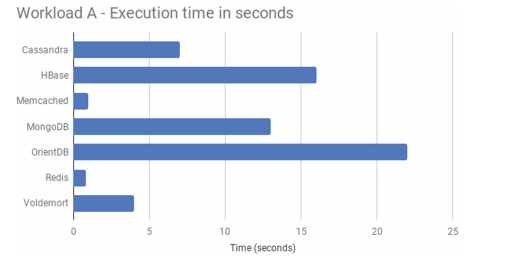
\includegraphics[width=0.9\linewidth]{figures/images/performance_a.png}
	\caption[6.000.000 rekord, 50\% olvasás, 50\% írás esetén]{\textit{6.000.000 rekord, 50\% olvasás, 50\% írás esetén}\footnotemark}
	\label{fig:performance_a}
\end{figure}

\footnotetext{https://www.researchgate.net/figure/Workload-A\_fig1\_332028074}

\begin{figure}[H]
	\centering
	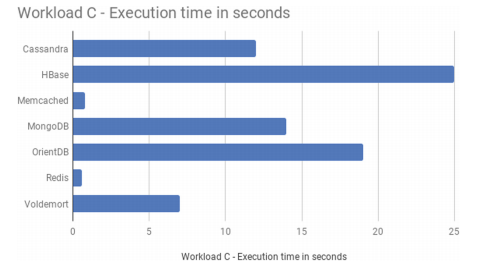
\includegraphics[width=0.9\linewidth]{figures/images/performance_b.png}
	\caption[6.000.000 rekord és 5.000 véletlenszerű olvasás esetén]{\textit{6.000.000 rekord és 5.000 véletlenszerű olvasás esetén}\footnotemark}
	\label{fig:performance_b}
\end{figure}

\footnotetext{https://www.researchgate.net/figure/Workload-C\_fig2\_332028074}

\begin{figure}[H]
	\centering
	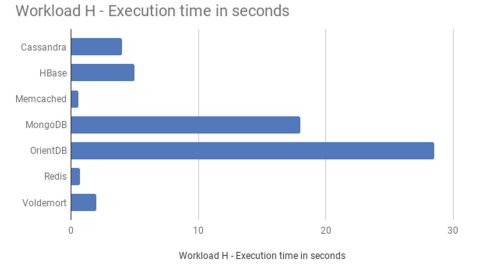
\includegraphics[width=0.9\linewidth]{figures/images/performance_c.png}
	\caption[6.000.000 rekord 5.000 véletlenszerű frissítés esetén]{\textit{6.000.000 rekord 5.000 véletlenszerű frissítés esetén}\footnotemark}
	\label{fig:performance_c}
\end{figure}

\footnotetext{https://www.researchgate.net/figure/Workload-H\_fig3\_332028074}

\section{Keretrendszerek}
	\paragraph{}
	A keretrendszerek napjainkban felkapott rendszerek lettek a felhasználók között. Ezek a rendszerek sokoldalúak, robusztusak és hatékonyak. A különböző alkalmazások fejlesztéséhez az ilyen jellegű rendszerek segítségével csak a magasabb szintű funkcionalitások elvégzésére kell koncentrálni. Erre az a magyarázat, hogy a keretrendszer gondoskodik az alacsonyabb funkcionalitásokkal. Számos előnyt lehet felsorolni, hogy miért jó ha használjuk ezeket a rendszereket.\cite{frameworks}
	\begin{itemize}
		\item Elősegíti a tervezési minták megfelelő kialakítását.
		\item Biztonságosabb kódolás.
		\item A redundáns kód elkerülése.
		\item Következetes kódfejlesztés kevesebb hibával.
		\item Megkönnyíti a kód tesztelését és a hibakeresést is.
		\item Az alkalmazás fejlesztéséhez szükséges idő lecsökken.
	\end{itemize}

	\subsection{Angular}
	\paragraph{}
	Az Angulart 2008-ban kezdték el fejleszteni a Google munkatársai. A fejlesztés JavaScriptben történt. Abban az időben a webhelyek többsége többoldalas alkalmazás megközelítésén alapult. Ennek viszont a teljesítménye az idő elteltével romlani kezdett mivel befolyásoló tényező lett az internet kapcsolat és a szerver reakció képessége is. Ezért létre hozódott az egy oldalas alkalmazások megközelítése ami abban segít, hogy a több oldalas weboldalak csupán egy oldalon jelennek meg. Az Angular volt az egy oldalas alkalmazások első kerete. Az egyik fő előnye, hogy a felhasználók egyszerű struktúrával kell dolgozzanak. Megtanulják az Angular sajátos felépítését ezáltal gyorsan és optimálisabban tudnak benne fejleszteni. Az sem elhanyagolható, hogy a fejlesztők egy részletes és egyértelmű dokumentációval szolgáltak a felhasználóknak. Egy TypeScript nyelv amely hasznos és könnyen használható. A TypeScript nyelvek nagyon elterjedtek lettek. \cite{wohlgethan2018supportingweb}
	
	\subsection{Vue.js}
	\paragraph{}
	A Vue.js(röviden: Vue) tekinthető a legújabb keretrendszernek. Hasonlít az Angularhoz. Mindkéttő TypeScript típusú. Használható kisebb, egyszerűbb projekteknél és egy komplexebb egy oldalas alkalmazás elkészítésénél is. Fő érdeme a skálázhatóság. Különlegessége, hogy egy nyílt forráskódú közösség fejlesztette ki, nem pedig egy nagyobb vállalat. Komponens alapú keretrendszer amely azt jelenti, hogy komponenseket különböztetünk és jelenítünk meg. Egy komponensen belül tudunk írni HTML, CSS és Script elemeket is. A megjelenítés egy oldalon történik ezért szükséges használni a útválasztást(rout).\cite{wohlgethan2018supportingweb}
	
	\subsection{Angular vs Vue.js}
	\paragraph{}
	Mindkét keretrendszernek megvannak az előnyei \ref{tab:table1} táblázat és a hátrányai is \ref{tab:table2} táblázat. 
	\begin{table}[H]
	\begin{footnotesize}
		\begin{center}
			\caption{Előnyök Angular és Vue.js között \cite{vuevsang} }
			\label{tab:table1}
			\begin{tabular}{p{2cm}|p{6cm}|p{6cm}}
				\textbf{Sorszám} & \textbf{Angular} & \textbf{Vue.js}\\
				\hline
				1 & TypeScript használata & TypeScript használata, részletes dokumentáció\\
				\hline
				2 & Részletes dokumentációval rendelkezik & Egy oldalas alkalmazások készítése \\
				\hline
				3 & Gyorsítja a fejlesztést & Könnyű integráció a meglévő struktúrákba \\
				\hline
				4 & & Kihasználja virtuális DOM előnyeit \\
				\hline
				5 & & Sebessége és rugalmassága optimális \\
			\end{tabular}
		\end{center}
	\end{footnotesize}
	\end{table}

	\begin{table}[H]
	\begin{footnotesize}
		\begin{center}
			\caption{Hátrányok Angular és Vue.js között \cite{vuevsang}}
			\label{tab:table2}
			\begin{tabular}{p{2cm}|p{6cm}|p{6cm}} 
				\textbf{Sorszám} & \textbf{Angular} & \textbf{Vue.js}\\
				\hline
				1 & Számos különféle struktúrát kínál, nehezíti a tanulást & Kevesebb erőforrást kínál\\
				\hline
				2 & Lassabb teljesítmény mert működik a reális DOM &  \\
			\end{tabular}
		\end{center}
	\end{footnotesize}
	\end{table}
	\paragraph{}
	Az előnyöket és hátrányokat figyelembe véve kerestem egy ábrát amely megmutatja, hogy a Vue.js és az Angular mennyire használatosak. \ref{fig:vueang} ábra figyelembe veszi az érdeklődés és elégedettségi arányokat. A bemutatott adatok alapján mindkét keretrendszert sokan használják. Javasolt a Vue.js egy komplexebb, összetettebb projekt megvalósítása esetén viszont Angularral is ellehet készíteni. Mindkettővel frontend részt készítenek a fejlesztők.
	
	\begin{figure}
		\centering
		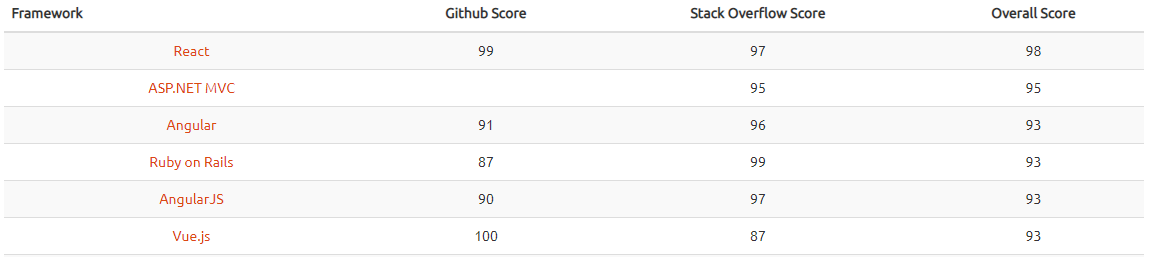
\includegraphics[scale=0.6]{figures/images/vueang.png}
		\caption{Keretrendszerek érdeklődési és elégedettségi szintjei évekre bontva \cite{vueanginterest}}
		\label{fig:vueang}
	\end{figure}
	
	\subsection{NodeJs}
	\paragraph{} 
	A NodeJs egy olyan szoftver platform, amely a Chrome V8 JavaScript futási idején épül fel. Fontos tulajdonsága, hogy skálázható ezért is sokan használják. Eseményvezérelt, nem blokkoló I/O modellt használ, amely könnyűvé és hatékonnyá teszi a valós idejű alkalmazásokhoz, amelyek elosztott rendszeren futnak át. Használatos mivel aszinkron és a tanulási görbéje is helyén van. A fejlesztők hatalmas köre már évek óta ismeri a JavaScriptet és az aszinkron programozást. Legtöbb esetben a NodeJs használatakor adatbázisnak NoSQL adatbázisokat választanak.\cite{js2016node}
	
	\subsection{Spring Boot}
	\paragraph{}
	A Spring Boot célja a Spring alkalmazás fejlesztés egyszerűsítése. Megtalálhatóak benne a következő tulajdonságok:
	\begin{itemize}
		\item Automatikus konfigurációk - Az alkalmazások Springként való működése érdekében.
		\item Indítófüggőségek - Biztosítja a felhasználóknak a szükséges függőségek(dependency) beimportálását. Ilyen lehet a Maven, Hibernate validátor, adatbázis eléréseket stb.
		\item Parancssori tolmács.
		\item Működtetés - A console-ba megjelennek az alkalmazás működésével kapcsolatos információk. Ilyen információ lehet a hiba, az elvégzett művelet stb.
	\end{itemize}
	
	\paragraph{}
	Radikálisan gyorsabb és széles körben hozzáférhető, érthető Spring fejlesztést nyújt. Számos funkciót kínál: beágyazott szervereket, metrikákat, ellenőrzéseket, külső konfigurációkat. Saját struktúrával rendelkezik és nem tesz különbséget az adatbázisok között. A JAVA nyelvet használja.\cite{jovanovic2017java}
	
	\subsection{NodeJs vs Spring Boot}
	\paragraph{}
	NodeJs a következő különlegességeket tartalmazza \cite{nodejsspring}:
	\begin{itemize}
		\item A NodeJS alkalmazások fejlesztésének elindítása könnyű.
		\item Az agilis fejlesztési módszertant követi, amely alkalmas a nagyon skálázható alkalmazásfejlesztési szolgáltatásokra.
		\item Nagy projekteknél gyorsabban működik mint a Java.
		\item Hatalmas erőforrás-készlet könyvtárakkal rendelkezik
	\end{itemize}
	
	\paragraph{}
	Spring Boot a következő különlegességeket tartalmazza \cite{nodejsspring}:
	\begin{itemize}
		\item Egyszerű, minden eszköz és operációs rendszer támogatja.
		\item Beépített nyelvbiztonsági funkciókkal rendelkezik, amelyeket a Java Compiler beágyaz.
		\item Robusztus kódot alkalmaz.
		\item Integrációs képesség jó.
		\item Az alkalmazások egyszerűen építhetőek fel.
		\item Beágyazott HTTP-kiszolgálókat, például Jetty, Tomcat használ és egyszerűen teszteli a webes alkalmazásokkal.
	\end{itemize}
	
	\paragraph{}
	A fent leírtakat figyelembe véve kerestem egy ábrát \ref{nodespring} amely az érdekeltségi szinetet mutatja meg.\cite{nodejsspring1} Mindkét keretrendszert inkább backend fejlesztésére használják.
	
	\begin{figure}
		\centering
		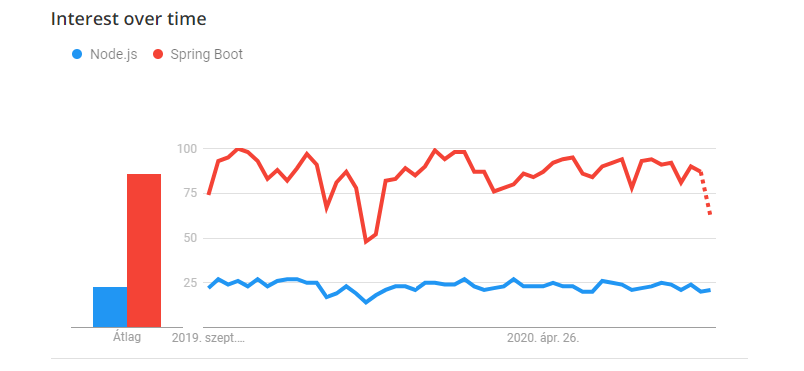
\includegraphics[scale=0.6]{figures/images/nodespring.png}
		\caption{NodeJS és SpringBoot érdekeltségi szintje}
		\label{nodespring}
	\end{figure}

\chapter{Követelmény specifikáció}
\section{Funkcionalitások}
	\paragraph{}
	Alkalmazásomon belül több fajta funkcionalitás jelenik meg. Első sorban nincs regisztrációhoz kötve a felhasználó. Ez azt akarja jelenteni, hogy mindenki előtt nyitva áll az alkalmazás. Viszont vannak különleges joggal rendelkező felhasználók, akik be tudnak jelentkezni és ennek következtében több funkcionalitást képesek használni.
	\paragraph{}
	Elsős sorban tisztázom, hogy a bejelentkező személyeket két csoportba különböztettem meg. Vannak admin és user felhasználók. Az admin felhasználó elér minden funkcionalitást. Az a jellegzetessége, hogy új felhasználót csak ő tud hozzá adni és csak ő tud törölni is. A hozzáadás úgy történik, hogy megad minden adatot és egy gombra kattintva az új adatok bekerülnek az adatbázis rendszerbe. Közben az új felhasználó fog kapni egy email-t amellyel eltudja fogadni a jelentkeztetést. Ügyelni kell, hogy az email érvényessége időhöz kötött. A törlés csak egyszerűen kiválasztással történik. Egyetlen felhasználó sem tudja törölni saját magát még az admin joggal rendelkezők sem.
	\paragraph{}
	A következőkben a user joggal rendelkező felhasználók lehetőségeit részletezem. Ezeknek az embereknek lehetőségük van hozzáadni új 3D modelleket az egyetemről, eseményeket, órarend linkeket és nem utolsó sorban az oldalon található fejléc képének módosítására is képesek. A tanszékek, szakok leírásának megadásai is lehetővé válik számukra. Sőt ha netán új szak indul azt is hozzá lehet adni.
	\paragraph{}
	A bejelentkező felhasználók számára természetesen van kijelentkező opció is. Ezen funkciók mellett a fejlesztés során, valószínűleg sokkal több lesz. Egyelőre a cél az egyszerűségben rejlik. Tudni kell, hogy a modellnél, tanszékeknél, szakoknál és más fontos információknál elérhetőségeknél mindig az adatbázisban szereplő legújabb adat jelenik meg. 
	\paragraph{}
	A következőkben tárgyalom a visitor(látogató) felhasználó által elérhető funkciókat. Az első és legfontosabb, hogy megjelenik egy 3D modell az egyetem épületéről amelyen a felhasználók tudnak nézelődni. Tudják nagyítani, kicsinyíteni, sőt még lehetőségük lesz arra is, hogy az épületet körbe tudják járni. 
	\paragraph{}
	Mindenki számára megjelenik a bejelentkezési lehetőség is. Viszont ezt a funkciót csak azok használhatják akik rendelkeznek felhasználónévvel és jelszóval.
	\paragraph{}
	A második legfontosabb funkció a tanszékek, szakok megjelenítése. Ez egy külön oldalon lesz. A felhasználók itt láthatnak egy leírást és az elérhetőségeket egy adott tanszékről. Ezek mellett egy útvonalat is megtekinthetnek a 3D modellen belül így amikor oda érkeznek az egyetemre nem kell annyira keresgélni, hogy mi hol található. 
	\paragraph{}
	Mindenki számára elérhető lesz az esemény naptár is. Ezen részen jelennek meg azok az események amelyeket az egyetem szervez a diákok részére. Látható lesz az események pontos dátuma, helyszíne, ára és itt is megjelenik egy olyan opció is amely a 3D modellen megmutatja az útvonalat. Ez azért jó mert ha egy idegen ember érkezik egy ilyen eseményre, például versenyre, akkor könnyebben elfog tudni igazodni, hogy hová is kell mennie.
	\paragraph{}
	Utolsó funkcionalitásnak egy vélemény nyilvánítást tettem be. 
	Itt minden felhasználó, név nélkül tudja közölni az alkalmazással kapcsolatos észrevételeit. Ha valaki véleményt szeretne írni akkor értékelnie is kell egy skálán, hogy szerinte mennyire hasznos az alkalmazás. A vélemények lehetnek pozitívak és negatívak is mindezek mellett új ötlet javaslatokat is lehet írni. Figyelembe véve a véleményeket lehetőség van jobbá fejleszteni az alkalmazást. A felhasználók nem csak véleményt tudnak nyilvánítani, hanem a mások által adottakat el is tudják olvasni. A vélemények szerkesztésére nem lesz lehetőség.
	\paragraph{}
	A funkcionalitásokból is látszik, hogy a céloknak megfelelően próbáltam megfelelni. Törekedtem az egyszerűségre átláthatóságra. Kiderült, hogy a regisztrációs rész nem egyedi módon történik meg. Az alkalmazás megpróbál minden olyan lehetőséget magába foglalni ami a diákok számára elérhető kell legyen.
\section{Felhasználói követelmények}
	\paragraph{}
	A Sapi3D alkalmazás web alapú, ezért mindenki számára elérhető
	a fő célja, hogy egy 3D modellként jelenítse meg a Sapientia EMTE Marosvásárhely-i karának a fő épületét, illetve ennek fontosabb helyeit, mint pl. tanszékek, titkárság stb.
	A rendszer fontosabb funkcionalitásait és az ezeket igénybe vevő szerepköröket a \ref{fig:UseCase} ábra szemlélteti.
	\paragraph{}
	A rendszer működése érdekében semmi előfeltételt nem kell teljesítenie a felhasználónak mivel a weboldal egyik része teljesen nyitott, elérhető bárki számára. A rendszer megértésének érdekében tekintsük meg a \ref{fig:UseCase} ábrát amely bemutatja a rendszer különböző részeit.
	\paragraph{}
	Az \ref{fig:UseCase} ábrát tekintve észre vehetünk három aktort amelyek különböző vagy ugyan azt a tevékenységet végezhetik el. Megfigyelhető, hogy a visitor(látogató) átváltozhat user felhasználóvá. Az admin felhasználó tulajdonképpen egy user felhasználó aki admin jogosultsággal rendelkezik. A user és admin típusú felhasználók azok a személyek akik az oldal karbantartásáért felelősek.
	\paragraph{}
	Bármely felhasználó, aki egy böngészőből megnyitja az oldalt, a látogató kategóriából került.Ez a fajta felhasználó megtekintheti a 3d modellt, körbe sétálhatja és el tud jutni pl.titkárságra. Amint megnyílt az oldal rögtön látható az egyetemről készített modell. Ezen a modellen tud nézelődni, esetleg körbe is tudja járni, vagy adott helységekre el is tud jutni(például: titkárság, adott tanszék). Ezen kívül lehetősége van információk, elérhetőségek, események részleteinek elolvasására is. Minden visitor(látogató) ugyan akkor leírhatja saját véleményét, meglátásait az oldallal kapcsolatban is. A fent említett műveletek elvégzéséhez nem kell sem bejelentkezés, sem regisztráció.
	\paragraph{}
	Amint már említettem a visitor(látogató) át tud alakulni user felhasználóra. Ez abban különbözik a látogatótól, hogy be is tud jelentkezni és több műveletet tud elvégezni. A műveletek elvégzésének engedélyezése azon múlik hogy a bejelentkező felhasználó user vagy admin. Ha user képes bejelentkezni, eseményeket megadni, az egyetemmel kapcsolatos információkat módosítani, új 3D modellt is hozzáadni. Ezeken kívül mivel jelen van bejelentkezés így a kijelentkezés opció is a rendelkezésükre áll.
	\paragraph{}
	A regisztrációs feladatot egy admin jogosultsággal rendelkező ember végezheti el. Nem csak a regisztrálás tartozik az ő feladatköreihez hanem a userek törlése is az ő feladata. Ezen plusz műveletek mellett szintén elvégezheti az user és a visitor műveleteit is.
	\begin{figure}
		\centering
		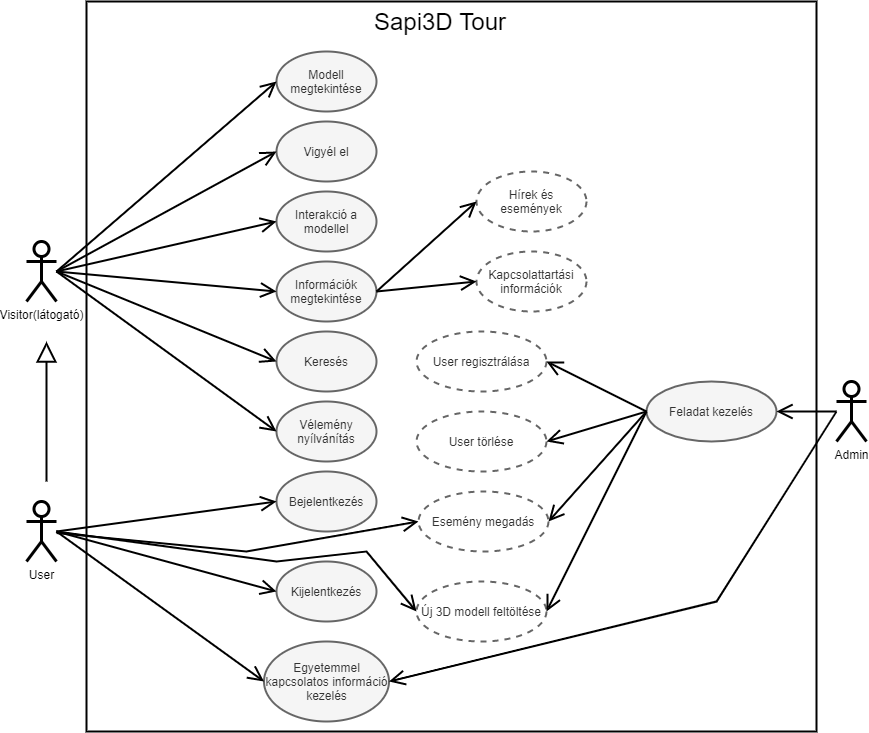
\includegraphics[scale=0.6]{figures/images/UseCase.png}
		\caption{Use Case diagram}
		\label{fig:UseCase}
	\end{figure}
\pagebreak
\section{Rendszerkövetelemények}

\subsection{Funkcionális követelmények}
\subsubsection{Visitor}
\begin{itemize}
	\item A használathoz a digitális eszköz lehet laptop, asztaligép, tablet vagy akár telefon is. 
	\item Interakció a 3D modellel a megjelenített gombok használatával. A gombok bíztosítják az előre hátra jobbra és balra menést.
	\item A "Vigyél el" funkció használata. A modell fölött található legördülő listából való kiválasztás esetén egy új gomb megjelenésével és annak használatával látható lesz az út a bejárattól a kiválasztott helyre.
	\item Fontos egyetemi helyek menüpont megtekintése, ahol az adatbázsban található adatok jelenítődnek meg. A címkre kattintva megjelennek a bővebb információt tartalmazó linkek. A címek mellet megjelenik egy térkép ikon is, amelyre ha rákattintanak akkor vissza kerülnek a 3D modellhez és a "Vigyél el" funkciót használva ismét megmutatódik az út a bejárattól a kiválasztott helyig.
\end{itemize}

\subsubsection{User}
\begin{itemize}
	\item Jelszó hitelesítése. Az e-mail-ben kapott validációs tokent felhasználva a jelszó hitelesítés oldalon megadni a jelszót, a megfelelő formátummal (Legyen benne legalább kisbetű, nagybetű és szám. Legyen legalább 5 karakter hosszú). Az e-mailben kapott validációs token lejárati idővel rendelkezik.
	\item Bejelentkezés a regisztrált e-mail és hitelesített jelszó megadásával történik, amint a User megnyomja a "Bejelentkezés" gombot.
	\item Hozzáférés az adatbázisban tárolt adatokhoz.
	\item User képes szerkeszteni a saját adatait (név, e-mail cím, telefonszám), ha rákattint a jobb sarokban lévő ember ikonra. Ezek után egy ablakba előjönnek az adatai amelyek szerkeszthetőek. A szerkesztés után a "Adatok szerkesztése" gombra kattintva az adatok bekerülnek az adatbázisba. A megadott adatok elegett kell tegyenek a megfelelő formátumoknak.
	\item Az egyetemi részleg megadása, szerkesztése funkciónál egy rádiógomb segítségével ki tudja választani a User, hogy új részleget szeretne megadni, vagy már egy létező részleget szeretne módosítani. Ha a részleg megadását választja akkor megkell adja a részleg nevét (példaul: Dékáni Hivatal) és egy {\textit{linket}\footnotemark} amely elvisz a részleget leíró oldalra. Ezek után a "Hozzáadás" gomb megnyomásával az adatok bekerülnek az adatbázisba. A szerkesztés esetén lehet módosítani a nevet is és a linket is. A "Szerkesztés" gomb segítségével az adatbázisban szereplő adatok átíródnak.
	\footnotetext{https://ms.sapientia.ro/hu/munkatarsak/dekani-hivatal}
	\item A szak megadása és szerkesztése funkciónál szintén egy rádiógomb segítségével tudja eldönteni, hogy megadni szeretne egy új szakot, vagy a meglévőket szeretné modósítani. Az új szak megadásánál a következő információkat kell megadni: szak neve; szakkoordinátor neve; szakkoordinátor e-mail címe; terem száma, ahol a szakkoordinátor tudja fogadni az érdeklődőket; egy lineket a szak részletes leírásához és egy legördülő lista segítségével, hogy melyik tanszékhez tartozik az adott szak. A "Hozzáadás" gomb segítségével az adatok bekerülnek az adatbázisba. A szerkesztés esetén a fent említett adatokat lehet szerkeszteni. A szerkesztés akkor lesz végleges ha a User megnyomja a "Szerkesztés" gombot.
	\item Egy részleghez, nem csak szakot lehet megadni hanem eseményeket, tevékenységeket is ha az Egyebek hozzáadását használja a User. Itt megkell adni egy legördülő lista segítségével, hogy a mely részleghez tartozik (például Villamosmérnöki Tanszék), egy nevet (például: Sapi-Line-Tracer), és egy lineket ahol több információ van leírva az eseményről, tevékenységről. Itt is szintén a "Hozzáadás" gomb megnyomásával kerülnek be az adatok az adatbázisba.
	\item A User ha elvégezte a hozzáadásos, szerkesztéses feladatait, akkor a jobb felső sarokban találahtó "Kijelentkező" gombra kattintva ki is tud jelentkezni.
\end{itemize}

\subsubsection{Admin}
\begin{itemize}
	\item Hozzáférés az adatbázisban tárolt adatokhoz.
	\item Userek regisztrálása és az adatok validálása a teljes név, e-mail cím, telefonszám megadásával. Az e-mail cím és a telefonszám eleget kell tegyen a megfelelő formátumoknak. A telefonszám csak számokból állhat és 10 karakterből kell álljon. Ezek után a "Hozzáadás" gomb lenyomásával az adatok eltárolása a NoSql adatbázisba és egy e-mail küldés a Usernek a jelszó hitelesítéséhez, amely tartalmaz egy validációs tokent, ami a regisztráció pillantában generálódik.
	\item Userek törlése: a User e-mail címének kiválasztása egy legördülő listából, majd a "Felhasználó keresése" gomb lenyomásával a User adatainak megkeresése. Ezek után a "Törlés" gomb használatával a User adatainak kitörlése az adatbázisból.
\end{itemize}

\subsection{Nem funkcionális követelmények}

\begin{itemize}
\item A rendszer használatához a felhasználóknak szüksége van Internetre és egy digitális eszközre amelyen megtudják nyitni a webalkalamzást. 
\item A felhasználók nincsennek egy adott operációs rendszerhez kötve. 
\item Az operációs rendszer lehet Windows, Linux, Android és iOS is. 
\item Külön telefonos applikáció még nincs, viszont a telefonokon található böngészők bármelyikében meglehet tekinteni az alkalmazást.
\item A regisztrált felhasználók adatai egy NoSQL adatbázisban (MongoDB) vannak eltárolva, amely nem lokálisan van jelen a felhasználók eszközén.
\item Az azonosítás a Spring Boot beépített autetikációs moduljával történik meg.
\end{itemize}

%Terv

\chapter{Architektúra}

%\chapter{Modulok leírása}
%\chapter{Adatbázis leírása}
%\chapter{UI terv}
%\chapter{Proiect menegment}
%\chapter{Verzió követés}

\chapter{Gyakorlati megvalósítás}
\section{Megvalósítások}
Első részben a megvalósításokat natív HTML CSS és JavaScript elemekkel próbáltam megoldani. Ez volt az az időszak amikor elkezdtem utána nézni, hogy a céljaim közül mi valósítható meg és mi nem. Az első amivel bővebben kezdtem foglalkozni maga a 3D modell betöltése volt egy web oldalra. Idő közben rájöttem, hogy natív HTML-be nem tudok beimportálni egy 3D objektumot. Kerestem keretrendszereket ahol tudok használni ilyen jellegű modelleket. Először Angular keretrendszerben próbáltam ki. Itt elég sok időt eltöltöttem, hogy megtudjam jeleníteni az objektumot de sikerült.

Tovább kutatva megtaláltam a Vue.js keretrendszert is. Ebben már egyszerűbb volt a 3D objektum beillesztése mivel az Angularhoz hasonlónak kellet volna lennie. Viszont Vue.js-ben találtam kimondottan egy csomagot(package) amely direkt ilyen jellegű modellekkel foglalkozott. Ezek után a 3D modell megjelenítése már hamar megtörtént. 

Ezt követően neki fogtam tanulmányozni, hogy mit is tudok kezdeni egy ilyen modellel. Első körben megtanultam betölteni a weboldalra. Majd tovább keresve már tudtam forgatni is az elemet. A közelítés és a távolítás alapból beépítve található a csomagban így ennek nem kellett utána keresnem.

A projektem egyik legfontosabb része, hogy egy 3D modellt tudjak beépíteni, kezelni lassan kezdett megvalósulni így elkezdtem készíteni egy demo-t ahol az elképzeléseimet próbáltam összeszedni, megjeleníteni. Ez egy hosszabb folyamatnak bizonyult viszont a végére kezdett körvonalazódni, hogy fog kinézni maga az alkalmazás. A demo elkészítését már csak Vue.js keretrendszeren belül készítettem el.

Mindezek után ráébredtem, hogy lassan neki kellene fognom az eredeti projektnek is. Így neki kezdtem lefejleszteni a demoban elképzelt ötleteimet. Először a visitor(látogató) felhasználók oldalát kezdtem elkészíteni. Itt rájöttem, hogy kellene nekem egy adatbázis és a backend rész is amely segítségével tudok az adatbázisban szereplő adatokkal dolgozni. Úgy döntöttem, hogy a frontend és backend részt párhuzamosan fogom elkészíteni.

Annak érdekében, hogy a frontend és backend részt tudjam párhuzamosan fejleszteni szükségem volt egy adatbázisra. Így neki fogtam elkészíteni az adatbázisomat. Először megterveztem a tábláimat majd megpróbáltam minden hibát kiküszöbölni. Úgy gondolom, hogy ezek a táblák még nem tökéletesek, lesz még változtatás rajtuk de egyelőre az elinduláshoz szükségesek. Az \ref{fig:database} ábrán láthatóak az adatbázis táblák. Láthatjuk, hogy kilenc tábla hozódott létre különböző kapcsolatokkal. Az admin tábla tartalmazza azokat a felhasználókat, amelyek be tudnak jelentkezni. A branch tábla tartlamzza a részlegket mint például a tanszékek, vagy a dékáni hivatal. Itt összeköttetés figyelhetünk meg két táblával is. A contactperson tábla megadja a kapcslattartó személyt míg a department tábla meghatározza a alrészlegeket mint például a szakok. Tovább tekintve láthatunk egy file nevű táblát ami fájlokat. Észrevehető, hogy ez a tábla is kapcsolatot teremt három különböző táblával. Az első tábla neve event amely már el is árulja hogy az eseményekhez kapcsolodó adatokat, információkat tartalmazza. A második tábla a headerimg amely a fejlécen megjelenő képet tárolja. Harmadik tábla a model amely maga a 3D modell-t leíró adatokat tárolja.
\begin{figure}
	\centering
	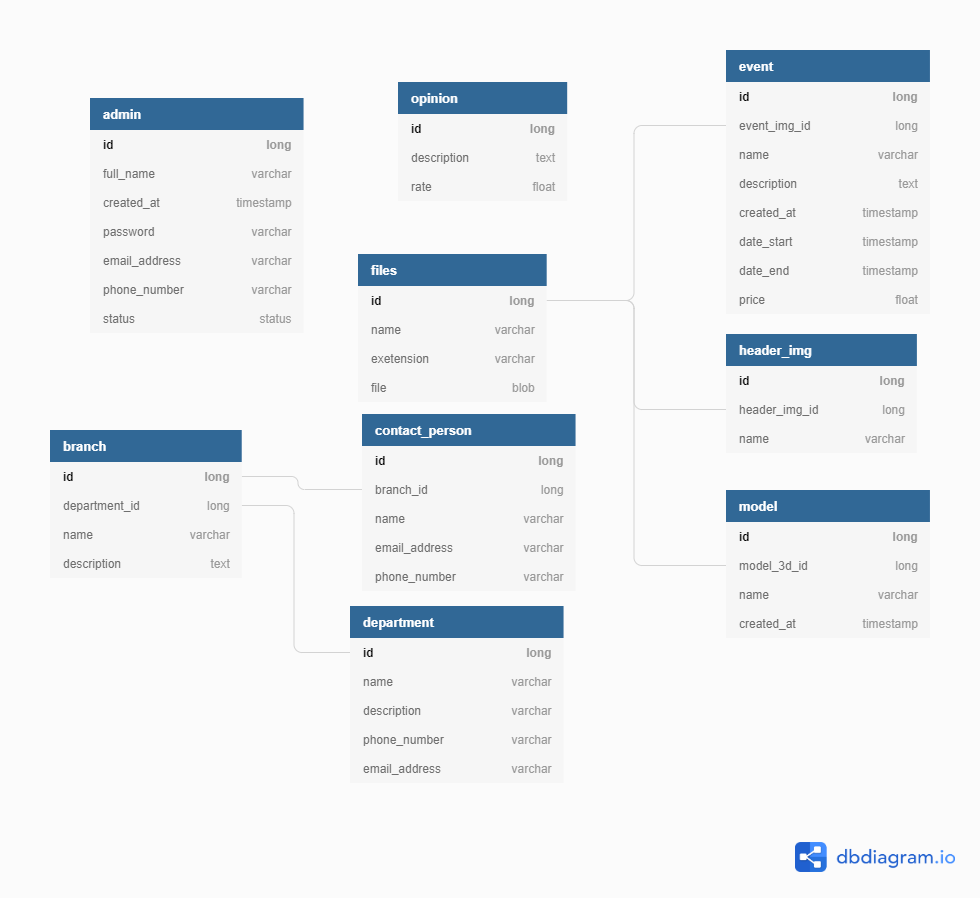
\includegraphics[scale=0.3]{figures/images/Sapi3dTour.png}
	\caption{Az adatbázist alkotó táblák.}
	\label{fig:database}
\end{figure}

Az adatbázis megtervezés után, neki fogtam a backend részt elkezdeni. Ehhez Spring Bootot használtam ami megkönnyíti az adatbázis létrehozásának folyamatát. A kódot Java-ban kell írni és minden tábla egy osztálynak felel meg. A Spring Boot tanulmányozása során jöttem rá, hogy mennyire oda kell figyelni a különböző annotációkra. Kis idő elteltével elsajátítottam a Spring Boot struktúráját és ezt használva felépítettem a backend rész első fázisát. Az adatbázis egyelőr PostgreSQL-ben van létrehozva viszont a Spring segítségével gyorsan bármely adatbázissal lehet kapcsolatot teremteni.

Mindeközben fejlesztettem a frontend részt is. Eljött az a pillanat, hogy kapcsolatot kellett teremtenem a frontend és a backend rész között, amelyet hamar sikerült elvégeznem. Így már tudott kommunikálni a frontend a backenddel vagyis a frontendre az adatbázisban szereplő adatok eljutottak és jelentek meg a weboldalon. 

A következő részben látható lesz képek formájában a forntend rész haladata. Az első részben bemutatnám, hogy a user felhasználók mit látnak. Első sorban a menürendszerrel kezdeném. Ha már be van jelentkezve egy felhasználó akkor a \ref{fig:drawbar} ábrán látható menü rendszerrel fog találkozni. Megfigyelhető, hogy megjelennek a felhasználó adatai és egy gomb amely segítségével tudja módosítani az adatait.Erről képet láthatunk a \ref{fig:changedata} ábrán. Ezek után jönnek a lehetőségek amelyekre rákattintva különböző oldalak jelennek meg.
\begin{figure}
	\centering
	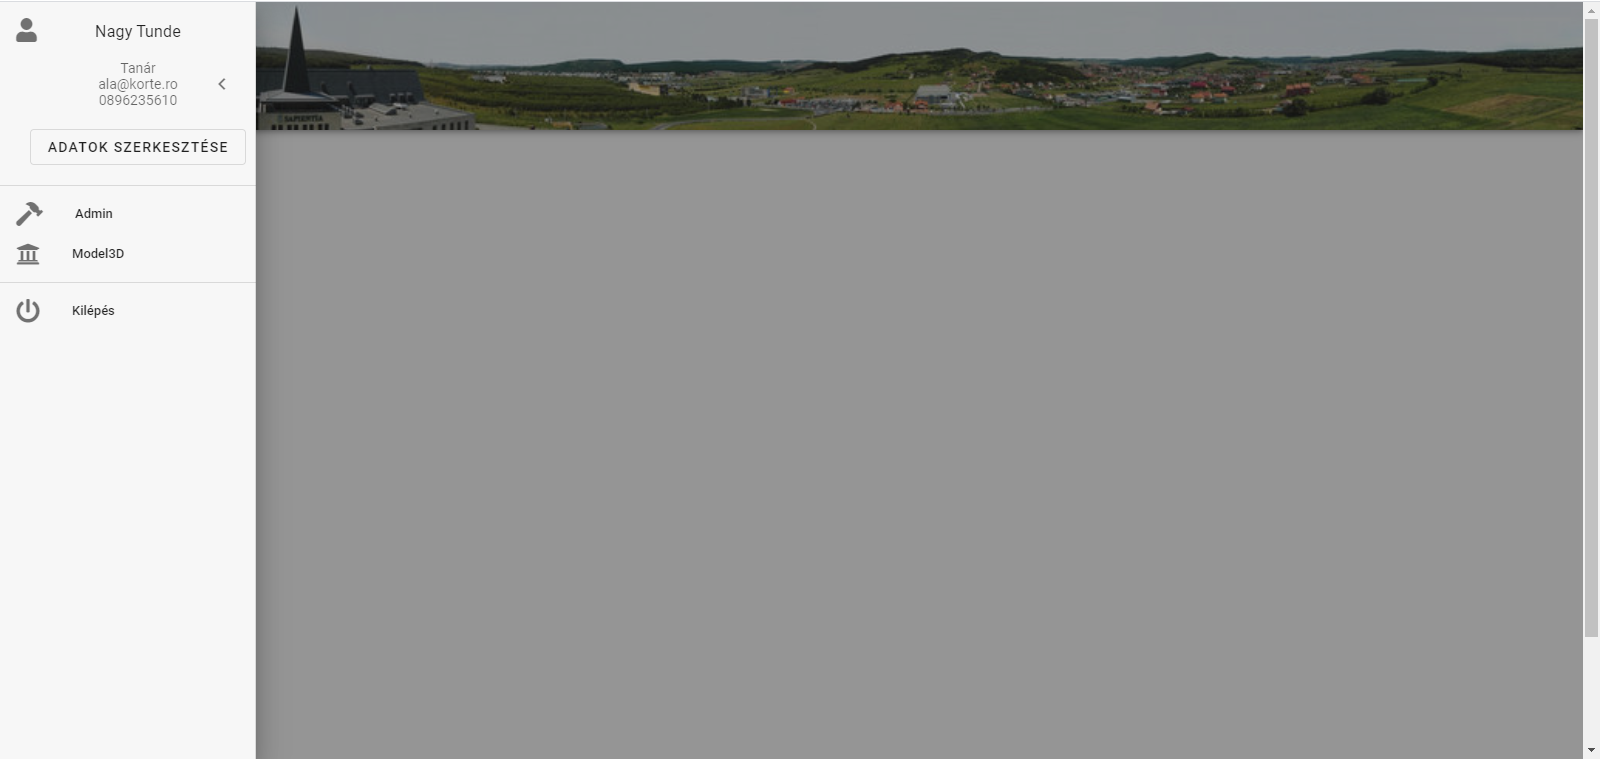
\includegraphics[scale=0.4]{figures/images/drawbar.png}
	\caption{A user felhasználók menü rendszere}
	\label{fig:drawbar}
\end{figure}
\begin{figure}
	\centering
	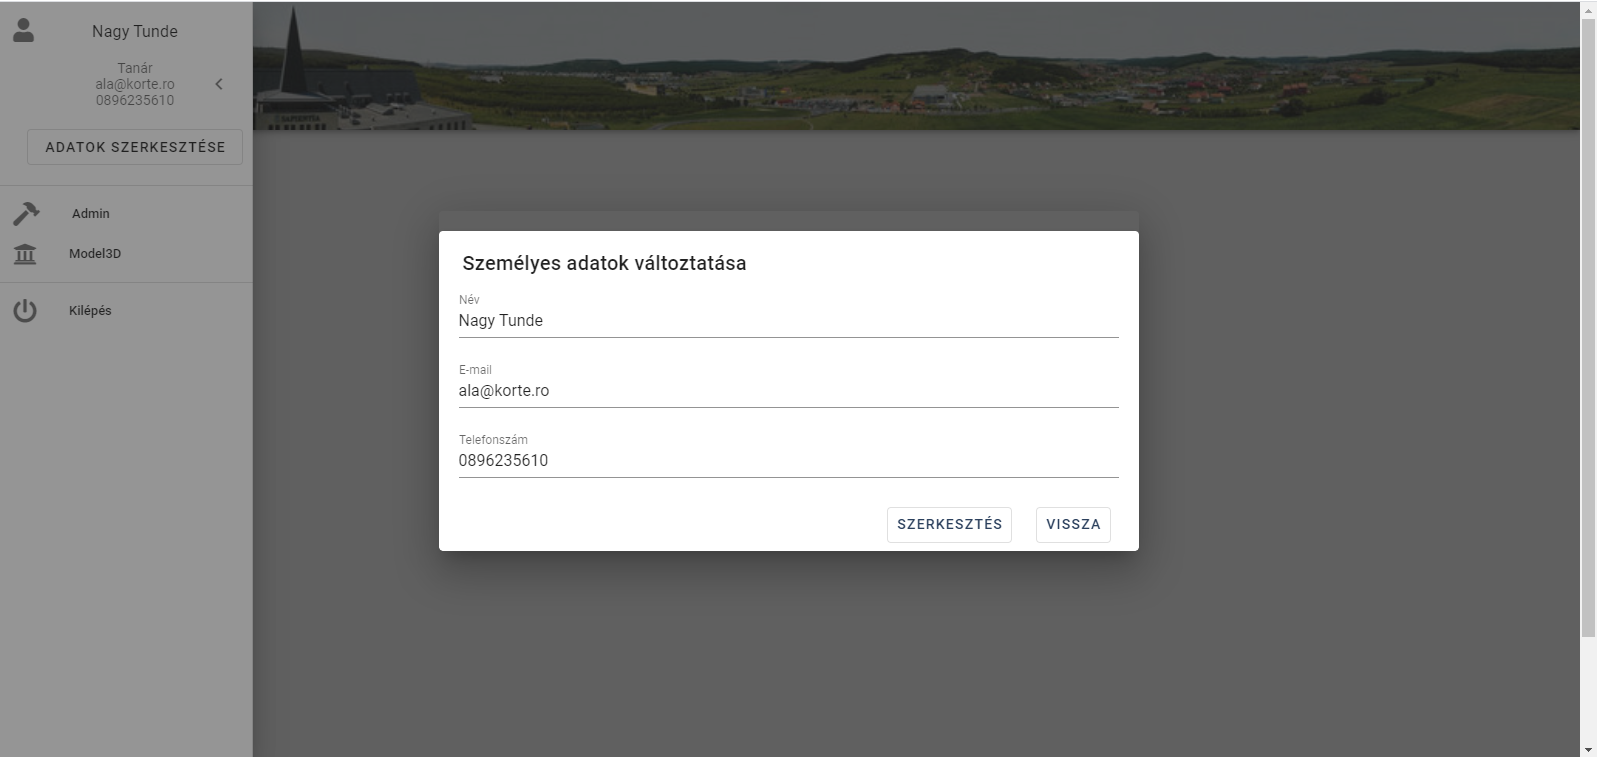
\includegraphics[scale=0.4]{figures/images/changedata.png}
	\caption{A user felhasználók adatainak módosítása}
	\label{fig:changedata}
\end{figure}
	
A menürendszer első opcióját választva vagyis az Admin opciót akkor előjönnek azok a funkcionalitások, amelyeket eltud végezni a felhasználó annak függvényében hogy milyen joggal rendelkezik. Egyelőre csak az új user felhasználók hozzáadása működik, amelyhez csak annyit kell tennünk, hogy beírjuk az adatokat és ráklikkelünk a HOZZÁADÁS gombra. Ez által bekerül az új felhasználó az adatbázisba. Erről az oldalról a \ref{fig:admin} ábrán láthatunk egy képet. Az utolsó menü pont a kijelentkezés gomb amely segítségével a felhasználó ki  tud jelentkezni és vissza kerül arra az oldalra amelyet már minden felhasználó képes látni.
\begin{figure}
	\centering
	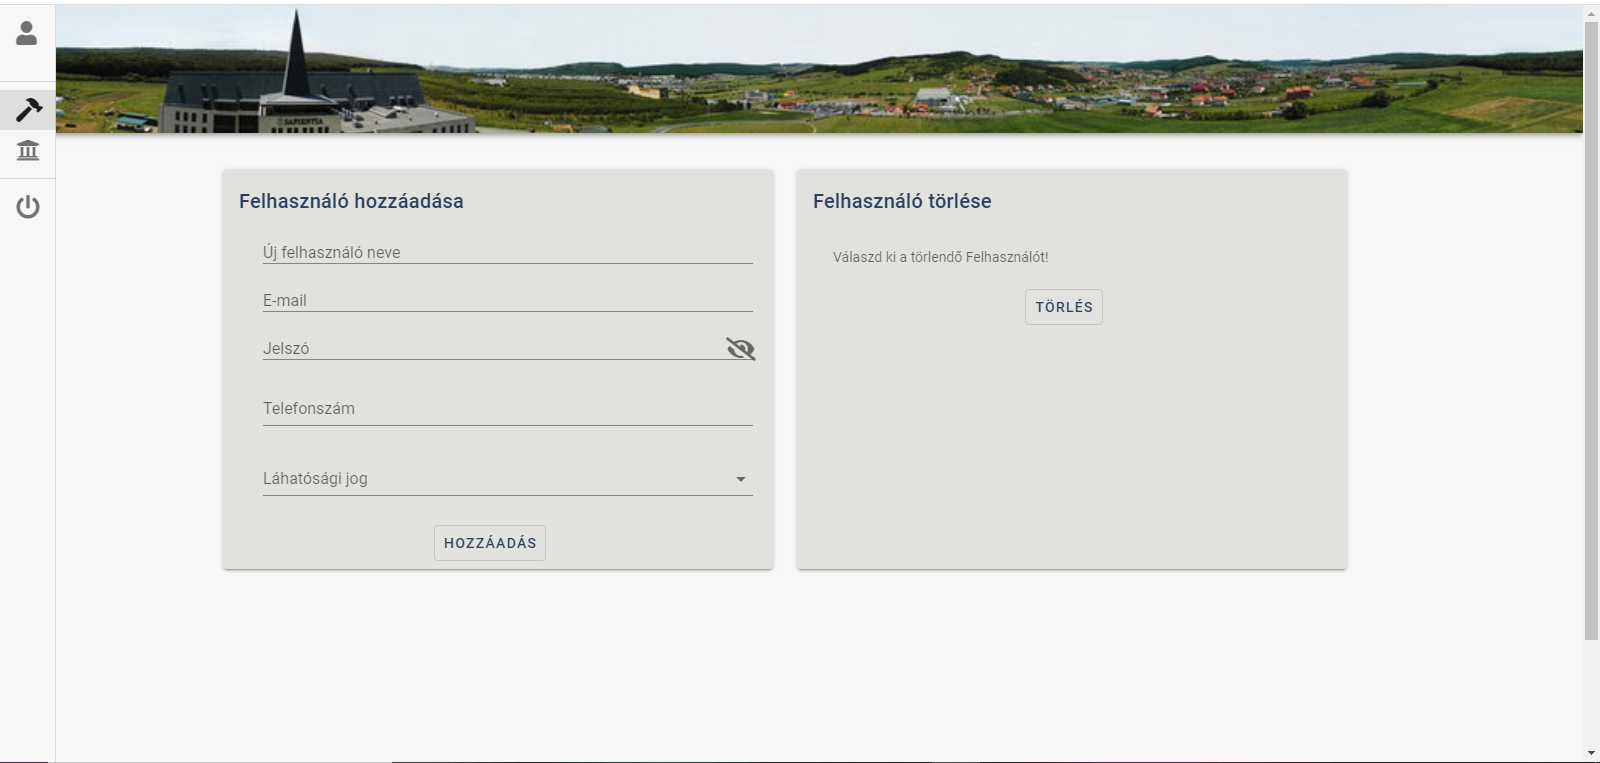
\includegraphics[scale=0.4]{figures/images/admin.png}
	\caption{A user felhasználók által használt különleges funkciók}
	\label{fig:admin}
\end{figure}
	
A következőkben azokat az elemeket mutatnám meg amelyeket minden felhasználó képes látni. Egyelőre csak egy ilyen oldal készült el és ez sem végeleges. Ezen az oldalon látható egy 3D modell amelyet a társam készített el. Megtekinthető a \ref{fig:modell} ábrán. Ezen kívül észrevehető, hogy ha nem vagyunk bejelentkezve akkor egy kicsivel másabb menürendszer jelenik meg. Ezt megtudjuk nézni a \ref{fig:drawbarevery} ábrán. A struktúra hasonló viszont itt nem jelennek meg a felhasználók adatai ámbár megjelenik a Bejelentkezés menüpont ahol be tudnak jelentkezni a felhasználók. Ez tulajdonképpen az útválasztás(rout) folyamaton belül oldódott meg. Egy útválasztás van és azon belül két nagyobb csoportra lett felosztva, hogy ki melyik oldalt láthatja. 
	
\begin{figure}
	\centering
	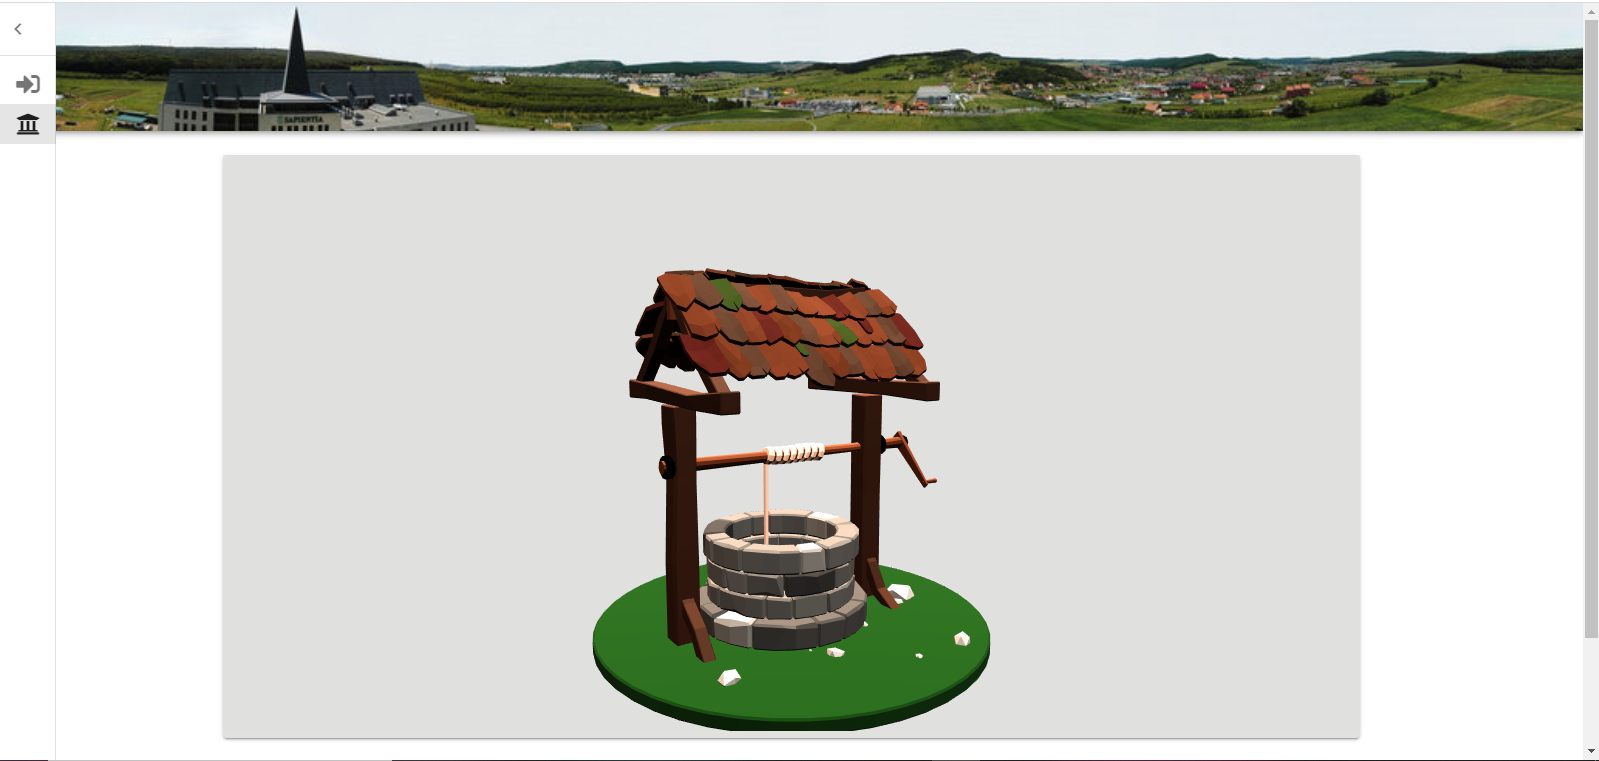
\includegraphics[scale=0.4]{figures/images/modell.png}
	\caption{A 3D modell kép visitor(látogató) és user felhasználók számára}
	\label{fig:modell}
\end{figure}

\begin{figure}
	\centering
	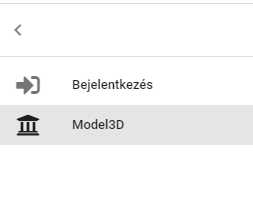
\includegraphics[scale=0.7]{figures/images/drawbarevery.png}
	\caption{Visitor(látogató) felhasználó által látható menürendszer}
	\label{fig:drawbarevery}
\end{figure}

Az alkalmazást egyelőre web felületen készítem el, mivel így a különböző eszközökön nem kell különbséget tenni. Nem kell megírni külön Android vagy IOS rendszerrel rendelkező mobiltelefonok nyelvére. A web felületre írt oldalakat megtudja nyitni az Androiddal és IOS rendszerre rendelkező ember is mivel nem kell külön alkalmazást letölteni. Ezen kívül egy weboldal elérhető számítógépen is. Fejlesztési lehetőségnek persze ott tartom azt is, hogy majd ne csak web applikáció legyen hanem Android meg IOS is. Mindkettőt hasznosnak tartom mivel világunkban a telefonok használata nagyon népszerű.

%következtetés
\chapter{Összefoglalás}
	\paragraph{}
	Az elmúlt nyár alatt ennyire sikerült az államvizsga projektemet fejlesztenem. Továbbra is törekszem, hogy minél jobban gyorsabban megoldjam a felmerülő problémákat. Folyamatosan próbálok ötletelni minél jobb és kreatívabb megoldásokról annak érdekében, hogy az alkalmazás hasznos legyen mint az egyetem és a diákok részére is. Úgy gondolom a nyár alatt elég sok mindent megtanultam, tapasztaltam a különböző rendszerekkel, technológiákkal kapcsolatban. Ezen tapasztalataimat nagy örömmel fogadtam és tudom, hogy majd a jövőbeni életemben is feltudom használni őket.

\addcontentsline{toc}{chapter}{Irodalomjegyzék}
\bibliographystyle{ieeetr}
\bibliography{References}

%appendix
%\appendix
%\chapter{Függelék}
%\section{Alfejezet}

\subsection{Cím}

\subsubsection{Alcím}




\end{document}